\chapter{Command \& Data Handling}%Worked on by Chris+Steph
\setlength{\parindent}{15pt}
\label{ch:avio_grou_hand} %Dont change this label (we know it does not adhere to the style)

In this chapter, the command and data handling is designed. This includes all UAV avionics and the general design of the ground station. First, in \autoref{sec:desi_appr_comm}, the design approach is illustrated in a flow chart. Then, in \autoref{sec:avio_grou_stat}, the avionics of the UAV are designed and in \autoref{sec:grou_hand_payl} the ground station is explained together with different payload modules. Finally, sections \ref{sec:comm_flow_diag}, \ref{sec:data_hand_bloc_diag}, \ref{sec:hw_sw_bloc_diag} and \ref{sec:elec_bloc_diag} show the communication flow diagram, data handling block diagram, hardware diagram, software diagram and last the electrical block diagram.
 
\section{Design Approach}
\label{sec:desi_appr_comm}
In \autoref{fig:comm_data_work} the design approach is visualised. 

\begin{figure}[htb]
    \centering
    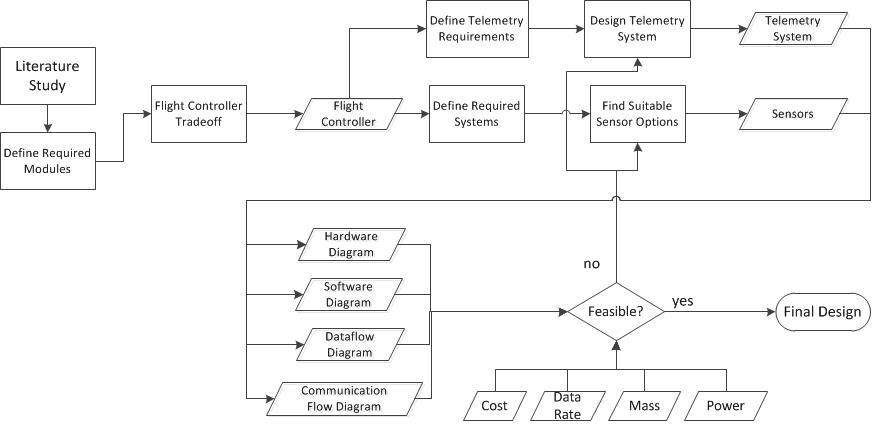
\includegraphics[width=\textwidth]{./CommandDataHandling/Figures/WorkFlow}
    \caption{Command and Data Handling Work Flow Diagram}
    \label{fig:comm_data_work}
\end{figure}



\section{Avionics}% and Ground Station}%Written by Steph, Chris + Steph responsible/worked on
\label{sec:avio_grou_stat}
In this section, all avionics used in the preliminary design will be explained. In order to cut down on cost as batch size increases, in future design stages some of the selected systems will be replaced by in-house designed systems. That would, however mean requirement SYS-OP-2.3 (that states the electrical components used should be off-the-shelf parts) has to be discarded.  

An overview of the systems that were selected can be found in \autoref{tab:avio_subs}. This was done based on the requirements in the SYS-OP category %(maybe refer to requirements)
and on extensive online research. Further specifications on the selected systems can also be found here. In \autoref{sec:avio_trad_off} a comparison is made between different available systems. The design of the telemetry system is discussed in \autoref{sec:tele_syst} and in \autoref{sec:grou_stat_layo} the layout of the ground station is explained. Then in \autoref{sec:encr} a secure communication protocol is established. 
\nomenclature[A]{GPS}{Global Positioning System}
\nomenclature[A]{BVLOS}{Beyond Visual Line of Sight}
%SUS-OP-2.3 the UAV shall be constructed with off-the-shelf electrical components use this for justifying pixhawk system
%&SYS-OP-2.5.3,4,5 Object avoidance, ground avoidance
%SYS-OP-2.7 Night conditions.......
%Include paparazzi STATE with software http://wiki.paparazziuav.org/wiki/Pixhawk
%Explain what is meant with modularity
%SYS-OP-2.9.2:The safe mode of the UAV shall have a return-to-base function.SYS-OP-2.9.3:autonomous emergency landing


\begin{table}[ht]
    \centering
    \caption{List of Avionics Subsystem Components}
    \label{tab:avio_subs}
    \begin{tabularx}{\textwidth}{>{\small}p{.15\textwidth} >{\small}p{.18\textwidth} >{\small}p{.12\textwidth} L}
    \toprule 
    \textbf{System type}     & \textbf{Selected system} & \textbf{Price} &\textbf{System specifications} 
    \\ \midrule
    Flight control module      & Pixhawk 2.1\footnotemark & USD 198,- & Isolated IMU (3x accelerometer, 3x gyroscope, 3x magnetometer, 2x barometer), flight controller board, multiple input ports, micro SD card for internal memory. Estimated size 10x5x2 cm, estimated weight 200 g. %this one goes last when all the others have been filled in
    \\ \hdashline
    Software            & Paparazzi\footnotemark & USD 0,- & Open-source, easy implementation of different functionalities
    \\ \hdashline
    Ground avoidance system & SF30-C Laser Rangefinder\footnotemark & USD 699,- & Range 100 m, accuracy $\pm$0.1 m, weight 35 g, dimensions 30 x 55 x 50 mm
    \\ \hdashline 
    Object avoidance system & Jenoptik DLEM 20\footnotemark & Estimated at EUR 1000,- & Sensor uses flight control module for avoidance of obstacles. Dimensions 50 mm x 22 mm x 34 mm, weight 33 g, range 5 km, accuracy 0.5 m.
    \\ \hdashline
    GPS & Here GNSS for Pixhawk\footnotemark & USD 48,- & Concurrent reception of up to three GNSS, -167 dBm navigation sensitivity, weight 49 g, dimensions 8x8x2 cm.
    \\ \hdashline
    2x Airdata sensors & Digital Airspeed sensor\footnotemark & USD 130 & 0.84 Pa resolution, Kit dimension 24x17x10 mm. Mounted at both wingtips. 
    \\ \hdashline
    Radio Control & Frsky V8FR-II receiver\footnotemark & EUR 14,- & 2.4 GHz, Weight 39g, dimensions 34x19x8 mm. \\
    & FrSky 2.4GHz Accst Taranis X9D PLUS\footnotemark & EUR 160,- & RC Transmitter for the ground station. 
    \\ \hdashline
    Telemetry & u-Blox TOBY L2-series \footnotemark &   EUR 60,- & Weight 4.8g, dimensions 25x36x3 mm.
    \\ \hdashline
    Payload link & USB or other cable & Estimated at EUR 10,- & Pixhawk module has multiple extra ports for both power and camera modules.
    \\ \midrule
     & Estimated total: & EUR 2200,- & Estimated total size: 400 cm$^3$, 400g.
    \\ \bottomrule
    \end{tabularx}
\end{table}


\addtocounter{footnote}{-9}
\stepcounter{footnote}\footnotetext{\url{http://www.robotshop.com/en/pixhawk-21-standard-set.html}, Accessed 12-06-2017}
\stepcounter{footnote}\footnotetext{\label{ft:pixhawk}\url{http://wiki.paparazziuav.org/wiki/Pixhawk}, Accessed 22-06-2017}
\stepcounter{footnote}\footnotetext{\url{http://www.robotshop.com/en/sf30-c-laser-rangefinder-100m.html}, Accessed 13-06-2017}
\stepcounter{footnote}\footnotetext{\url{https://www.jenoptik.com/products/defense-and-security/laser-rangefinders/oem-modules-system-integration/dlem}, Accessed 13-06-2017}
\stepcounter{footnote}\footnotetext{\url{http://store.jdrones.com/digital_airspeed_sensor_p/senair02kit.htm}, Accessed 21-06-2017}
\stepcounter{footnote}\footnotetext{\url{https://www.unmannedtechshop.co.uk/here-gnss-module-for-pixhawk-2/}, Accessed 22-06-2017}
\stepcounter{footnote}\footnotetext{\url{https://hobbyking.com/en_us/frsky-v8fr-ii-2-4ghz-8ch-receiver-hv.html}, Accessed 20-06-2017}
\stepcounter{footnote}\footnotetext{\url{https://hobbyking.com/en_us/frsky-2-4ghz-accst-taranis-x9d-plus-digital-telemetry-radio-system-mode-2.html}, Accessed 22-06-2017}
\stepcounter{footnote}\footnotetext{\url{https://www.u-blox.com/en/product/toby-l2-series}, Accessed 19-06-2017}

\begin{comment}
http://www.robotshop.com/en/uav-drone-sensors.html
http://pixhawk.org
http://www.robotshop.com/blog/en/how-to-make-a-drone-uav-lesson-4-flight-controller-15191
\end{comment}


\subsection{Trade-off}
\label{sec:avio_trad_off}
In this section, different options for the flight control and positioning systems are discussed. The systems need to be able to measure axial and angular accelerations, orientation, attitude, altitude, distance to the ground, distance to obstacles and determine its global position. The communication system will be discussed in \autoref{sec:tele_syst}.


In \autoref{tab:flig_cont}, an overview of (combinations of) systems is given that can determine all previously mentioned aspects and are able to process some data from for example monitoring equipment. For some of the systems the exact size or weight is not known. In these cases, sizes are either estimated based on reviews an images or not given when this was deemed too inaccurate. %FOOTNOTE EXPLAIN TRADE OFF TABLE AND OUTCOME EXPLAIN CHOICE OF GROUND AVOIDANCE SYSTEM AND OBJECT AVOIDANCE SYSTEM
This overview is then used to perform a trade-off between the different system layouts. First, weights were determined. The CPU has been assigned with the greatest weight factor, since it is the driving factor in a lot of missions. Size (weight and dimensions), modularity (the amount of available connections) and accuracy have been given equal weights. They are considered very important, however not as significant as the CPU. Size can make it very hard to carry the module and could pose some severe constraints on the structure, modularity is essential to the connection of different controllers and monitors yet in most boards, it is possible to overcome this by installing intermediate connectors, and accuracy is essential to the control of the UAV. Then cost, GPS and software were assigned with the smallest weight. The cost of all of the systems was found to be within the budget limits, a separate GPS system could be added in case the current system is not accurate enough, and software modules could also be changed. Then each of the concepts has been graded per criterion, where `- -' means that performance is extremely poor, `0' means average and `+ +' means very beneficial to the design or system. Then based on these weights and scores, the systems have been assigned with a grade that was found by adding or subtracting the weight factors as the scores stated it, then dividing by two and adding 40. That means scores between -15 and 105 are theoretically possible, yet all scores are between 0 and 100. The range was made larger (than from 0 to 100) to make different scores more outspoken.




\begin{table}[ht]
    \centering
    \caption{Overview of Flight Control Systems}
    \label{tab:flig_cont}
    \begin{tabularx}{\textwidth}{>{\small}p{.12\linewidth} L  >{\small}p{.13\textwidth}  }
    \toprule
\textbf{System(s) }     & \textbf{Specifications }       &\textbf{Price, Size}                                %& \textbf{Positives, Negatives}                                                                                        
\\ \midrule
Navio2 Autopilot, Raspberry Pi 3                       & GNSS receiver, extension ports, includes power module, dual IMU, 10 cm resolution barometer, 14 PWM servo outputs, 1.2GHz 64-bit quad-core ARM Cortex-A53 CPU, Integrated 802.11n wireless LAN and Bluetooth 4.1, software still required.                                                                                                                                                                                                                                                                                  & USD253,   2x   55x65x15 mm, 68g                                  % & Provides all desired ports for extra equipment, processor is strong enough. Software still needs to be designed.                                                             
\\ \hdashline             
Radiolink PixHawk 1             & 32bit STM32F427 Cortex M4 corewith FPU, 256KB RAM, 3-axis IMU, 16 bit gyroscope, 14 bit accelerometer and magnetometer. Size estimated.                         & USD140, 100x40x20 mm, 100g                                     %& GPS already included, relatively cheap. Possibly requires extra ports. Also IMUs processing capacity could be better. Software available 
\\ \hdashline
Lynxmotion Quadrino     & Nano Drone/UAV Flight Controller, Software included, IMU, Explansion ports, ATmega 2560 (256Kb flash @ 16MHz) Processor.                                                                 & USD150, 53x53x17 mm                                                                                                                           %& Software included.  Meant for smaller category drones, processor might not be able to handle it.    GPS included                                                                  
\\ \hdashline 
MWC MultiWii  & 2 Servo output for camera (only available when using 4 motors or less), Separate 3.3V and 5V LDO voltage regulators.                                                                                                                                                                                                                                                & USD23,      36x36x2 mm                                                                                                               %& Small, cheap.  Output/input port and processing capacity too small, arduino required..                                                                                              
\\ \hdashline
AfroFlight Naze32 Rev6                   & Up to 8 ch RC input, 32-bit processor running at 3.3V/72MHz. BMP280 barometer.                                                                                                & USD21,      36x36 mm,                                                                             7.3g  %& Small, cheap. Meant for quadcopter racing -- not suitable for a lot of data processing.                                                             
\\ \hdashline
DJI Naza-M V2                        & Software included,  Intelligent Orientation Control, PPM, S-BUS \& Ordinary Receiver Supported, Built-in Gimbal Stabilisation Function, Remote Gain Adjustment, Hovering Accuracy (GPS Mode) Vertical:$\pm$0.8m, Horizontal:$\pm$2.5m .                                               & USD 159,   4x  45x45x10 mm, 95 g             
                %& Software available, function extensions possible, GPS included. Not very accurate, not certain if CPU can handle all camera data. Relatively large.                              
\\ \hdashline 
Pixhawk 2.1, Here+ GNSS                    & Modular design for flexibility, Triple Redundant IMU system, Modular cube. All inputs/outputs in one single DF17 connector, Concurrent reception of up to three GNSS, -167 dBm navigation sensitivity.                                                                                                                                        & USD246, GPS 79x82x17 mm, 49g 
% & Has a lot of modular options which is ideal for the different payload modules. Also has good processing memory and availability to put in an external memory card.  Relatively large, however would still fit in the design.   
\\ \hdashline
Paparazzi           & Open source software and hardware, all required components can be installed, manuals available.    Hardware cost and size estimated.         &USD100, 50x50x10 mm, 50g
\\ \bottomrule
    \end{tabularx}
\end{table}











\begin{table}[ht]
    \setlength\extrarowheight{5pt}
    \setlength\arrayrulewidth{1pt}
    \centering
    \caption{Flight Control Trade-Off}
    \label{tab:avio_trad_off}
    \begin{tabular}{r|
    |>{\centering}p{1cm}
    |>{\centering}p{.5cm}
    |>{\centering}p{2cm}
    |>{\centering}p{1cm}
    |>{\centering}p{.5cm}
    |>{\centering}p{1cm}
    |>{\centering}p{.5cm}
    | c } 
    \raggedright \textbf{Concept \rotatebox{90}{\hspace{0.5cm}Criterion}}        & 
    \rotatebox{90}{\textbf{Size}}                            &
    \rotatebox{90}{\textbf{Cost}}                                   & 
    \rotatebox{90}{\textbf{CPU}}                            & 
    \rotatebox{90}{\textbf{Modularity}}                        & 
    \rotatebox{90}{\textbf{GPS}}                       &
    \rotatebox{90}{\textbf{Accuracy}}                         &
    \rotatebox{90}{\textbf{Software}}       &
    \rotatebox{90}{\textbf{Result}}
    \\\hline
    Navio2      &
    \cellcolor[HTML]{FFC000}-    &
    \cellcolor[HTML]{FFC000}-    &
    \cellcolor[HTML]{00B050}++   &
    \cellcolor[HTML]{00B050}++   &
    \cellcolor[HTML]{92D050}+    &
    \cellcolor[HTML]{92D050}+    &
    \cellcolor[HTML]{FFC000}-    &
    \cellcolor[HTML]{92D050}\textbf{78}
    \\[5pt]\hline
    Pixhawk 1          &
    \cellcolor[HTML]{FFFF00}0    &
    \cellcolor[HTML]{FFFF00}0    &
    \cellcolor[HTML]{92D050}+    &
    \cellcolor[HTML]{00B050}++   &
    \cellcolor[HTML]{92D050}+    &
    \cellcolor[HTML]{92D050}+    &
    \cellcolor[HTML]{92D050}+    &
    \cellcolor[HTML]{92D050}\textbf{70}
    \\[5pt]\hline
    Lynxmotion      &
    \cellcolor[HTML]{92D050}+    &
    \cellcolor[HTML]{FFFF00}0    &
    \cellcolor[HTML]{FFFF00}0    &
    \cellcolor[HTML]{92D050}+    &
    \cellcolor[HTML]{92D050}+    &
    \cellcolor[HTML]{00B050}++   &
    \cellcolor[HTML]{92D050}+    &
    \cellcolor[HTML]{FFFF00}\textbf{65}
    \\[5pt]\hline
    MultiWii       &
    \cellcolor[HTML]{00B050}++   &
    \cellcolor[HTML]{00B050}++   &
    \cellcolor[HTML]{FF0000}- -   &
    \cellcolor[HTML]{FF0000}- -   &
    \cellcolor[HTML]{FFC000}-    &
    \cellcolor[HTML]{FFFF00}0    &
    \cellcolor[HTML]{00B050}++   &
    \cellcolor[HTML]{FF0000}\textbf{28}
    \\[5pt]\hline
    Afroflight   &
    \cellcolor[HTML]{00B050}++   &
    \cellcolor[HTML]{00B050}++   &
    \cellcolor[HTML]{FF0000}- -   &
    \cellcolor[HTML]{FFC000}-    &
    \cellcolor[HTML]{FFC000}-    &
    \cellcolor[HTML]{FFFF00}0    &
    \cellcolor[HTML]{FFC000}-    &
    \cellcolor[HTML]{FF0000}\textbf{25} 
    \\[5pt]\hline
    DJI Naza M   &
    \cellcolor[HTML]{FF0000}- -   &
    \cellcolor[HTML]{FFFF00}0    &
    \cellcolor[HTML]{92D050}+    &
    \cellcolor[HTML]{92D050}+    &
    \cellcolor[HTML]{00B050}++   &
    \cellcolor[HTML]{FF0000}- -   &
    \cellcolor[HTML]{92D050}+    &
    \cellcolor[HTML]{FFC000}\textbf{43} 
    \\[5pt]\hline
    Pixhawk 2.1   &
    \cellcolor[HTML]{FFFF00}0    &
    \cellcolor[HTML]{FFC000}-    &
    \cellcolor[HTML]{00B050}++   &
    \cellcolor[HTML]{00B050}++   &
    \cellcolor[HTML]{00B050}++   &
    \cellcolor[HTML]{92D050}+    &
    \cellcolor[HTML]{92D050}+    &
    \cellcolor[HTML]{00B050}\textbf{80} 
    \\[5pt]\hline 
    Paparazzi &
    \cellcolor[HTML]{92D050}+   &
    \cellcolor[HTML]{FFFF00}0   &
    \cellcolor[HTML]{00B050}++  &
    \cellcolor[HTML]{00B050}++  &
    \cellcolor[HTML]{00B050}++  &
    \cellcolor[HTML]{00B050}++  &
    \cellcolor[HTML]{00B050}++  &
    \cellcolor[HTML]{00B050}\textbf{95}  
    \\[5pt] \hline\hline
    Weight          &
    10              &
    5              &
    20              &
    10              &
    5              &
    10              &
    5           &
    \\[5pt]
    \end{tabular}
\end{table}









From \autoref{tab:avio_trad_off} it can be seen that the MultiWii and Afroflight system are not suitable for this UAV. The DJI Naza M also underperforms, however, not as much as the other two. On the other hand, the Pixhawk 2.1 and the Paparazzi system are the winnners of this trade-off, closely followed by the Navio2 system. Solely based on the trade-off, the most logical option to choose the Paparazzi system. However, this system also has open-source hardware, which means it still needs to be built. Requirement SYS-OP-2.3 states, however, that all electrical components should be off-the-shelf. The Paparazzi system is not qualified as such, and therefore, the hardware used will be the Pixhawk 2.1. Since the Paparazzi software does allow for easy adaption as it is open-source, this will be used instead of the Pixhawk software. Paparazzi software is easily implemented on the Pixhawk module\footnote{See footnote \ref{ft:pixhawk}.}.




%It was decided to use a ready-to-use flight control system, instead of installing the different components separately. Therefore, the system needs to consist at least  of an inertia measurement unit (IMU) or accelerometer plus gyroscope to determine accelerations, a compass or magnetometer to determine orientation, a pressure meter and a system that measures the distance to the ground, and preferably a Global Positioning System (GPS). In order to decrease the chance of burnout, a power brick is included in the Pixhawk module to transform the battery voltage to the flight controller voltage and to monitor the battery properties. For object avoidance, two laser sensors will be installed. One with a short range for ground detection, and one able to scan objects that are very far away, for collision avoidance.






\paragraph{Object Avoidance} The object avoidance system was selected after the flight control module. Initially, a trade-off would be performed on these as well. Both a ground sensor as well as a sensor that functions as the `eyes' of the UAV needed to be selected. For these sensors, different options are available. Some options and their (dis)advantages can be seen in \autoref{tab:obje_avoi}. Based on this comparison and the need for a sensor that can detect objects located up to 3 km away (Requirement SUB-AV-3.2), laser rangefinders were found to be the most suitable option. Some research was done on suitable laser rangefinders, and it was found that especially for the object avoidance, not a lot of options were present. The selected ground detection system was the cheapest one within  acceptable sizes and acceptable detection range (Requirement SUB-AV-3.3), while the selected object detection system was the only one that was within acceptable size limits while being able to detect objects very far away (Requirement SUB-AV-3.2). The specifications on these systems can be found in \autoref{tab:avio_subs}.



\begin{table}
    \centering
    \caption{Object Avoidance Sensor Types\protect\footnotemark }
    \label{tab:obje_avoi}
    \begin{tabularx}{\textwidth}{>{\small}p{.11\textwidth} >{\small}p{.4\textwidth} L}
    \toprule \bfseries
    Type        & \bfseries Advantages            & \bfseries Disadvantages
    \\ \midrule
    Laser rangefinder     
    & Ranges varying from 10 cm to up to 25 km. Laser has to return, yet does this at the speed of light making it very fast.
    & Accuracy comes at high cost. Eye-safety must be taken into account meaning not all lasers can be used (only class 1 and 2)\footnotemark
    \\ \hdashline
    LIDAR       
    & Very accurate.
    & Complete 3D surfaces can be mapped, which means more CPU is used than required for the purpose, expensive, large, heavy.
    \\ \hdashline
    Infrared
    & Cheap, direct response, can also be used at night.
    & Very sensitive to sunlight.
    \\ \hdashline
    Doppler radar
    & Used more often in aviation.
    & Measures relative velocity, not distance; signal needs to bounce back.
    \\ \hdashline
    SONAR
    & Can also detect very small objects.
    & Very expensive, large.
    \\ \bottomrule
    \end{tabularx}
\end{table}





\addtocounter{footnote}{-2}
\stepcounter{footnote}\footnotetext{\url{https://www.intorobotics.com/types-sensors-target-detection-tracking/}, Accessed 20-06-2017}
\stepcounter{footnote}\footnotetext{\url{https://www.rli.com/resources/articles/classification.aspx}, Accessed 20-06-2017}



\subsection{Telemetry System}%Made by Chris
\label{sec:tele_syst}

In this section, the Radio Control, (RC), system used for Visual Line of Sight, (VLOS), is discussed. Then, different possible telemetry systems for BVLOS communication are introduced and a final system is chosen.

\nomenclature[A]{VLOS}{Visual Line of Sight}

\paragraph{VLOS}

In order to control the drone in VLOS, a RC receiver is added to the telemetry system of the drone. The main purpose of this receiver is to obtain flight commands send by the operator while in VLOS. These flight commands are send directly to the UAV and are used in order to change thrust and provide control over the different control surfaces. This means, the operator can control the deflection angles and mangitude of thrust directly via the controller. 

Although the long range telemetry system in the next section could also be used for this purpose, a RC sender is preferred in close range due to the lower latency (as a direct link is established between operator and drone). Also the reliability of an RC link is higher, as the codes are not modulated and package loss is decreased due to the closer range.     

One disadvantage of the RC link is the fact that it is only used as a one-way link. Measurements of the different sensors are not send towards the ground station and hence it is only used for VLOS control. Data gathered on-board the UAV is send using the cellular link or has to be stored on the internal memory in case the cellular link breaks or is not available.

The most common RC link uses a 2.4 GHz frequency. Comparing different 2.4 GHz receivers, it was concluded, that a Frsky V8FR-II receiver will be used\footnote{\url{https://hobbyking.com/en_us/frsky-v8fr-ii-2-4ghz-8ch-receiver-hv.html}, Accessed 19-06-2017}. It uses eight channels, four used to simultaneously control rudder (change in yaw angle), elevator (change in pitch angle), throttle (change in thrust) and ailerons (change in roll angle). One remaining channel is then used for the tilting mechanisms of the engines, making it possible to manually transition from vertical to horizontal flight. The last three channels can be used for different payload modules which might require some kind of control, this can included opening and closing of the payload bay, rotating of cameras or dropping of payload. In case none of these are necessary, it can be decided that the three remaining channels are coupled to the 4 engine tilting mechanisms separately. This makes it possible to control the rotation of a single engine and can be used for control in vertical flight for example.



\paragraph{BVLOS}

The main requirement set for the BVLOS telemetry system is given by requirement SYS-PF-1.3, stating that the UAV, shall be capable of achieving a range of 200 km. As radio frequency communication can not reach these ranges, 2 alternatives are presented in this section: 
\nomenclature[A]{RC}{Radio Control}




\begin{enumerate}
\item{\textbf{Satellite Modem}}

In order to increase the range, a satellite modem could be used. This first sends the data towards a satellite which in turn redirects it towards the drone. The main advantage is that most areas of the Earth are covered and BVLOS operation is thus possible. Using a satellite modem, there are no range limitation. Major disadvantage is the  higher latency, as propagation and processing delays can be up to one second for a geostationary satellite connection. Furthermore, costs for using a satellite link are expensive and data rate dependant. Comparing only the dataflow of the sensors, a constant flow of up to 65 kbps can be necessary (see \autoref{sec:data_hand_bloc_diag}). Using the Iridium satellite network, this results in a cost of around 6 euro per second transmitting all the relevant data, which does not include yet live video feeds or other data consuming devices mounted in the payload.\footnote{\url{http://www.rock7mobile.com/products-rockblock}, Accessed 19-6-2017}

\item{\textbf{GSM/LTE Modem}}

Global System for Mobile Communications (GSM) and Long Term Evolution (LTE) modems make use of mobile cellular networks for the data transfer. As mobile telecommunications are widely available nowadays, using a GSM/LTE modem greatly increases the range compared to a radio modem. On top of that, data rates of up to 50 Mbps can be achieved in good conditions.\footnote{\url{https://www.u-blox.com/sites/default/files/TOBY-L2_DataSheet_\%28UBX-13004573\%29.pdf}, Accessed 12-6-2017} Although this makes it possible to use BVLOS operation, cellular networks are less developed in poorer countries and do not cover the oceans at all. This reduces the possible operational area significantly compared to satellite networks. The cost of data services is relatively low compared to satellite links. Several distributors in the Netherlands provide 10 GB of data transfer for around EUR 30,- per month.\footnote{\url{https://www.kpn.com/mobiel/mobiel-internet/simkaart/mobiel-internet-standaard/1-jaar}, Accessed 19-6-2017} 
\end{enumerate}
\nomenclature[A]{GSM}{Global System for Mobile Communications}
\nomenclature[A]{LTE}{Long Term Evolution}
Although the higher coverage of satellite communication is preferred for save and rescue missions, the cost is limited and high data transfer is required in order to obtain a reliable video feed for monitoring. Furthermore, satellite communications require bigger antennas in order to achieve a safe and reliable data connection. Another major advantage of using cellular networks is the fact that the packages are send using conventional networking technologies and hence also routed this way. This makes it easier to securely deliver the messages, which is in more detail explained in Section \ref{sec:encr}. For these reasons, a GSM/LTE modem is used as larger range telemetry system. This then also comes with the advantage that in order to control and monitor the drone only an internet connection is necessary.

The chosen GSM/LTE modem is a u-Blox TOBY L2-series LTE Modem. It can be connected directly to the Pixhawk Flight Controller via UART. Care should be taken that the correct module is chosen depending on the geographical location where the drone is operating. 

\paragraph{Final Layout}

Finally, the UAV uses a cellular network connection as main telemetry system. Via an internet connected device, waypoints can be send to the telemetry module for navigation. The flight controller then chooses the best control inputs to perform the mission. Furthermore, higher data rates are supported using this connection, hence also attitude data and monitoring data is send on this channel.

A second, more reliable link is created using the RC connection. This connection can only be used for lower ranges (up to 2 km) and hence it is only used for VLOS. Using the RC channel, the operator can control the thrust as well as pitch, yaw and roll angles. Transitioning from vertical to horizontal flight will also be possible using the controller. RC communication is thus preferred in case a higher precision is required, as position determination is dependant on GPS accuracy. 

In case the flight controller receives messages from both links, the newest messages are preferred and performed. Furthermore, in case the main cellular link breaks, the flight controller tries to establish a connection with the RC transmitter. If no link is available within 10 seconds, a return to take-off procedure is performed during which the UAV aborts its mission and returns to its starting point. 






\subsection{Encryption}%Made by Chris
\label{sec:encr}

The UAV market is increasing significantly without a major consideration in the safety of the exchanged messages. This comes with the problem that an adversary can without major troubles control the drone. 

A secure communication should be confidential (only the receiver can read the message), authenticated (the receiver is sure who sent the message) and integer (nobody can change the message). However for the flight control communications of the drone it is of no relevance whether an adversary knows that the drone is going to perform a certain action, this section only focuses on authentication and integrity. In case data has to be confidential, it is recommended to look into different encryption techniques using less processing power. 

The protocol used for flight control message exchange is the Micro Air Vehicle Communication (MAVLink) protocol. It is used for internal communication between the different sensors and the flight controller as well as to transmit useful information as attitude, speed and battery status of the vehicle and to send new waypoints for control of the drone. Although the integrity of the messages is already ensured by the checksum, it only has a length of 2 bytes (16 bits). This checksum can be guessed easily by current computers and hence the scheme is not secure.
\nomenclature[A]{MAVLink}{Micro Air Vehicle Communication}
Integrity and authentication are obtained using a Message Authentication Code (MAC). Before the MAVLink data is send to the cellular network, a Hash-based message authentication code (HMAC) is attached to it. In order to prevent replay attacks, the current time and date will also be added to the message before calculating the MAC. The HMAC uses the same principles as the checksum explained before, however, it can only be calculated knowing a symmetric key, stored at both the internal memory of the ground station and the drone.  Furthermore, the length of the checksum is equal to 16 bits, a HMAC however can have a length of 128 bits, making it more secure. This scheme is only secure if no third party is able to access either the drone or the ground station. Regular exchange of the key improves the security of the system.
\nomenclature[A]{MAC}{Message Authentication Code}
\nomenclature[A]{HMAC}{Hash-based Message Authentication Code}


The preceding encryption algorithm makes sure that the drone does not accept any commands send by an unauthenticated device. Furthermore random noise errors and messages that have been interfered with are also discarded. The final message send over the cellular network is depicted in \autoref{fig:encr_mess}. Due to the fact that the cellular network is used to transmit the message, an IP header is added in front of the MAVLink message, which includes beside others routing information. It can size from 20-60 bytes depending on the optional fields. The MAC is added at the end of the message and is calculated using only the orange fields, the MAVLink Frame and the Time and Date (T/D).

\begin{figure}[htb]
    \centering
    
\includegraphics[width=\textwidth]{./CommandDataHandling/Figures/encryption}
    \caption{Final Message Layout}
    \label{fig:encr_mess}
\end{figure}






\section{Ground Handling and Payload}%made by Steph
\label{sec:grou_hand_payl}

In this section, some relevant aspects related to the ground handling are discussed: the payload mounting mechanism and the possible payload modules, as well the ground station layout.


\subsection{Ground Station Layout}%made by Steph
\label{sec:grou_stat_layo}
%what kind of data is shown on the ground station? And what functionalities are required? Without defining these, you can't justify any choice of hardware/software.



In this section, the different options for the ground station are discussed, after which a layout for the system is chosen. %maybe mention requirements
Before selecting a layout, the functionalities of the ground station are defined. This is done based on different aspects of the UAV missions.
\begin{description}
    \item[Automated flight control] The location of the UAV shall be displayed, as well as its velocity, heading and altitude. It shall also be possible to see the flight plan. Besides that, waypoints can be added and the destination can be changed. The battery percentage shall also be shown.  
    \item[Manual fligth control] Since the UAV is in VLOS, showing its location is redundant here. However, battery, attitude, heading and velocity are useful parameters and shall therefore be shown. It shall be possible to give directional inputs, that cause accelerations. 
    \item[Mission specific capacities] When a camera module is present in the payload, the recorded shall be visible on the ground station. The payload status shall also be visible, so whether a payload is present or not. In the case of a disposable payload, the payload bay closing mechanism must be operated. Therefore, in that case the status of the mechanism shall be shown, and it shall be possible to open or close it from the ground station.
\end{description}




The two categories to choose between are a large ground station with a case, displays and controls, or just software that can be installed on any tablet or laptop with an internet connection. It was decided that using software is preferred, since it allows for more flexibility in interfaces, which is beneficial for the variation of mission types. Also, a tablet is easier to transport. Furthermore, as cellular technology is used for communication, only an internet connection is required for control. The only disadvantage is that the UAV will have to rely more on the autopilot, because the inputs given on a tablet will not be control inputs, but waypoints. After some research on world network coverage, it was decided that using just software and a tablet is a viable option\footnotemark. However, to have manual control in VLOS, a RC controller is used. This will be incorporated in the system.
\footnotetext{\url{http://data.worldbank.org/indicator/IT.CEL.SETS.P2?view=map}, Accessed 12-06-2017}



It was decided to choose a system that is compatible with the Pixhawk system that was selected in \autoref{sec:avio_grou_stat}. Therefore,  Paparazzi software will be used\footnotemark. It is compatible with the Pixhawk, all sensors and equipment connected to it can be incorporated in the program because of the open-source character of the software.

\footnotetext{See \autoref{ft:pixhawk}.}

Then, in order to use the more reliable RC Link, as explained in \autoref{sec:tele_syst}, an RC transmitter is needed. A FrSky ACCST TARANIS X9D PLUS Digital Telemetry Radio System\footnotemark  is used for this, since it is recommended to use with the Pixhawk module and its pricing fits within the avionics and ground station budget. It supports at least the 8 channels available by the RC receiver and can hence be used for direct control of the aircraft.

\footnotetext{\url{https://hobbyking.com/en_us/frsky-2-4ghz-accst-taranis-x9d-plus-digital-telemetry-radio-system-mode-2.html}, Accessed 19-06-2017}



\subsection{Payload Mounting}

In this section, the payload mounting mechanism will be explained. For the closing mechanism of the fuselage, please refer to \autoref{sec:payl_bay_clos_syst}.


Since some missions require a droppable payload module, the mounting mechanism should allow for this. There also are cases in which it would be beneficial to only drop part of the payload, making it possible to take extra batteries or camera equipment. This means two things:

\begin{description}
\item[Modular payload] In order to enable for part of the payload to be dropped, it is possible to put in different pieces of payload, as long as they fit in 15x15 cm with varying lengths, and the total length of the payload modules does not exceed 1 m. In order to keep fragile payloads from shaking, magnets will be used.  
\item[Releasable payload] The payload will be mounted using a clipping system. Each module will have rigid bars, disposable ropes or something else that allows the module to be held. This is then clipped to a system that works similar to nippers. The `nippers' are mounted to two parallel bars, like in \autoref{fig:payl_moun_syst}.(3), and can be operated individually by the CPU. 
\end{description}

\begin{figure}
    \centering
    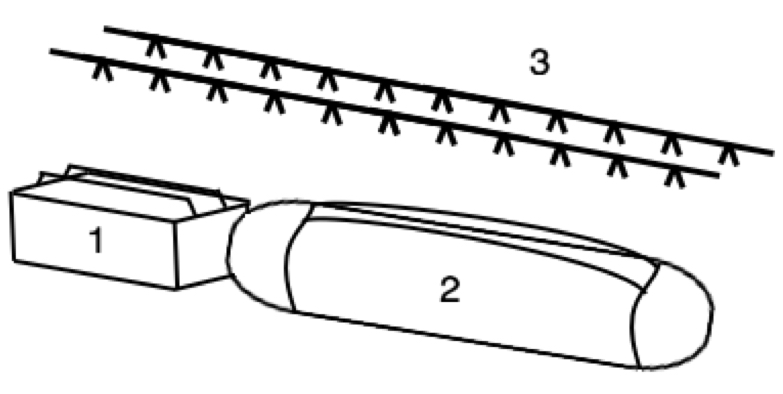
\includegraphics[width = .5\textwidth]{CommandDataHandling/Figures/Payload_module}
    \caption{Schematic Example of Payload Mounting System}
    \label{fig:payl_moun_syst}
\end{figure}







\subsection{Payload Bay Closing System}
\label{sec:payl_bay_clos_syst}
In this section, the closing mechanism of the payload bay is explained. In the midterm report, no intentions were expressed of incorporating such a system \cite{midterm}. However, since for some missions, (part of) the payload will be released from the fuselage, it needs to be possible to close the fuselage to prevent excessive drag. The possibility of closing the fuselage also allows for different payload shapes to be transported without extra packaging.


To determine how the system would look, first some brainstorming was done. Different options were swinging doors, sliding doors, a mechanism in which the door would be positioned above the payload, and a roller system. Each of these systems has advantages and disadvantages. In \autoref{tab:fuse_clos_comp}, some of these are listed. 

\begin{table}[ht]
    \centering
    \caption{Comparison of Different Fuselage Closing Mechanisms}
    \label{tab:fuse_clos_comp}
    \begin{tabularx}{\textwidth}{>{\small}l L L}
    \toprule
    \textbf{System} & \textbf{Negatives} & \textbf{Positives}
    \\ \midrule
    Swinging doors & Difficult to transfer stresses, extra connecting mechanism is required. Heavy. Large. &  Closes automatically as payload is dropped.  
    \\ \hdashline
    Sliding doors & Difficult to transfer stresses, extra connecting mechanism is required. Heavy. Large. &  Closes automatically as payload is dropped.
    \\ \hdashline
    Fall-down door & Heavy. Large. & Can transfer stresses. Closes automatically as payload is dropped. 
    \\ \hdashline
    Roller system & Requires an additional rolling system. & Can include bars to transfer stresses. Light as it can be partially made out of fabric. Compact.
    \\ \hdashline
    Discard entire module & Very unsustainable. Only closes the fuselage before release; this is actually not a closing mechanism. & Can transfer and sustain stresses considerably better than the other systems. 
    \\ \bottomrule
    \end{tabularx}
\end{table}


It was decided that the most important aspect in the design of the closing was the ability to help the rest of the fuselage sustain stresses. This is because if the bottom of the fuselage can not transfer any stresses, the whole design needs to be a lot stronger. Based on this, the decision was made to make a distinction between constant and in-flight removed payload.

\begin{description}
    \item[Constant payload] This is a payload module that is not dropped. Because a compete payload module can sustain a lot more stresses than a separate closing mechanism, as the walls of such a module also carry loads, in the missions that not require dropping the payload a closed box is used, like in \autoref{fig:payl_moun_syst}.(1).
    \item[Droppable payload] In the case of a payload that needs to be delivered in-flight, a separate small payload module is installed that closes the fuselage after payload release. This module will be installed next to the payload that is dropped, so that it only covers that part of the fuselage that needs to be closed. It will consist of a small box with dimensions 15x15 cm times the diameter of the rolled-up closing sheet. This shall be a roller system which consists of fabric to reduce the drag and bars to carry strength. Within the closing module, a small motor is present that operates the unwinding of the sheet. The module shall be connected to the CPU so that it closes the fuselage right after the payload is dropped.
\end{description}








\subsection{Payload Modules}
In this section, a short discussion on suggested payload modules for the different mission profiles will be given. The payload modules \textit{will not} be designed into full detail; however, components such as cameras are preferably chosen such that they are easily compatible with the Pixhawk flight control system. A modular clicking system will be installed, so that it is possible to drop (part of) the payload.

\begin{enumerate}
\item	\textbf{Search and rescue and support to disaster relief operations.} This requires a module that is able to locate the person(s) in need, and drop a help module. The difficulty in this module is that it will be dropped, so if an extra camera or battery is needed, those should be put in a separate module. As the object avoidance system that was chosen in \autoref{tab:avio_subs} only shows presence without being specific, some camera should be taken or dropping location would be based on GPS. The payload then only contains of a care package or buoy. Velocity and range are most important here, but a mission specific trade-off should be made between that performance and payload capacity.
\item	\textbf{Precision agriculture by monitoring of cattle and crops.} For this type of mission, high-quality camera equipment is required. Endurance is the most important feature for this mission type, so an extra battery will also be installed. A camera that takes images at a high frequency should be selected, so it is possible to still generate lift using the wings.
\item \textbf{Transportation of parcels at sea and on land.} This type of mission requires large range. Therefore it will probably make use of a separate battery payload module and parcel module, where maximum battery size is dependent on payload size.
\item \textbf{Inspection of extensive industrial assets and infrastructures such as railways, high-tension powerlines, pipelines, wind farms, etc.} This type of mission requires similar equipment as mission 2. The difference is that this mission type documents long-range objects, while the agricultural one should cover large areas. Therefore, range is very important in this mission type. It will also make use of high-quality camera equipment and if possible and extra battery module.
\item 	\textbf{Transportation of organs for transplants.} In the case of transporting organs, high velocity is very important. The payload should be well-protected, which means it will probably be light, yet large. Some room might be available for extra batteries. The payload will not be dropped, but the UAV will land for unloading, so a cooling case could be designed for this means.
\end{enumerate}


\section{Communication Flow Diagram}
\label{sec:comm_flow_diag}

In this section, the communication flow diagram is illustrated in \autoref{fig:comm_flow_diag}. It illustrates the flow to and from the UAV system to the environment. 

\begin{figure}[ht]
    \centering
    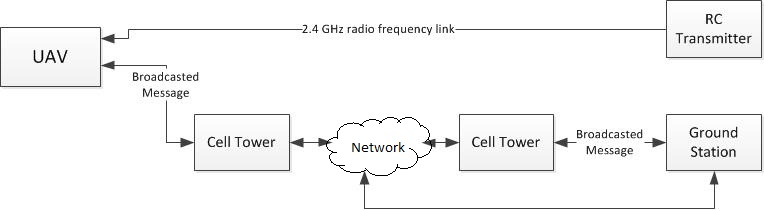
\includegraphics[width=.8\textwidth]{./CommandDataHandling/Figures/CommFlowDiagram.jpg}
    \caption{Communication Flow Block Diagram}
    \label{fig:comm_flow_diag}
\end{figure}

As explained in \autoref{sec:tele_syst}, the telemetry system consists of two different links, a direct link between the UAV and the control station using radio frequency and an indirect link using cellular technology. The radio frequency link is a one-way link to only send control commands to the flight controller. These commands are send using Pulse Width Modulation (PWM) techniques. As seen in \autoref{fig:comm_flow_diag}, data send using the mobile network is first broadcasted through the air until it reaches a cell tower. Using the routing information on the IP packet, the data is either routed directly towards the ground station (in case it is connected to the internet) or to the closest cell tower from the ground station (in case it is connected via the mobile network). In the latter case, the cell tower broadcasts the message and the ground station can receive it. The data send via the mobile network range from monitoring data to new waypoint or commands send to the drone to change its flight path. 

\nomenclature[A]{PWM}{Pulse Width Modulation}

\section{Data Handling Block Diagram}
\label{sec:data_hand_bloc_diag}

In this section, the data handling block diagram is depicted in \autoref{fig:data_hand_bloc_diag}. The main purpose of this diagram is to illustrate the different data flows across the system. Furthermore it depicts the sample rates and processing speeds. 

\begin{figure}[ht]
    \centering
    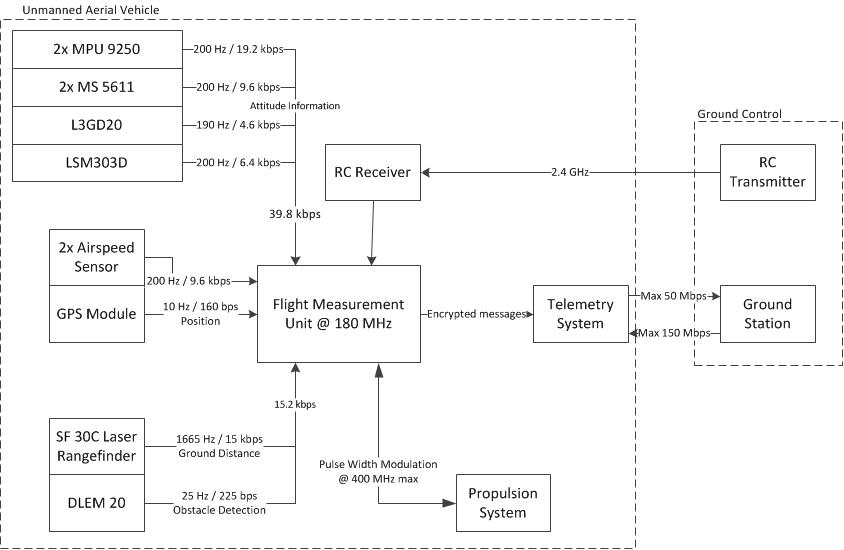
\includegraphics[width=0.8\textwidth]{./CommandDataHandling/Figures/DataDiagram.jpg}
    \caption{Data Handling Block Diagram}
    \label{fig:data_hand_bloc_diag}
\end{figure}

The attitude sensors can sample the information at different rates, however more sampling results in a bigger data flow and higher required processing power. It was assumed that sampling attitude information at a speed of 200 Hz results in a good overview of the UAV attitude. The sampling rates for the object avoidance, ground distance and GPS measurements are set to their maximum sampling rate. As no specification have been obtained until now considering the sampling rate of the airspeed sensor, it is also assumed to sample at 200 Hz. The frequency at which commands can be send to the propulsion system is limited by the physical link, in this case 400 MHz, which can however never be achieved due to the bottleneck set by the flight measurement unit of 180 MHz. The down- and uplink speeds of the telemetry system are their maxima and only achievable if the network is not congested. 

All sensors (position, attitude and object/ground avoidance) have a total data rate of 65 kbps. Some minor headers are added to the packages after processing due to the message authentication code and routing information, however the end data rate is orders of magnitude lower than the total achievable rate of 50 Mbps. This means enough margin is provided for the payload data rate and minor network congestion.   


\section{H/W \& S/W Block Diagrams}
\label{sec:hw_sw_bloc_diag}

In this section, the hardware and software diagrams are represented in Figures \ref{fig:hwdia} and \ref{fig:swdia}. As can be seen, they are are closely related. The hardware diagram focuses on the different physical interfaces used in the UAV and shows the different types of link between each interface. The software diagram illustrates the software that processes the data of each interface. 

\begin{figure}[ht]
    \centering
    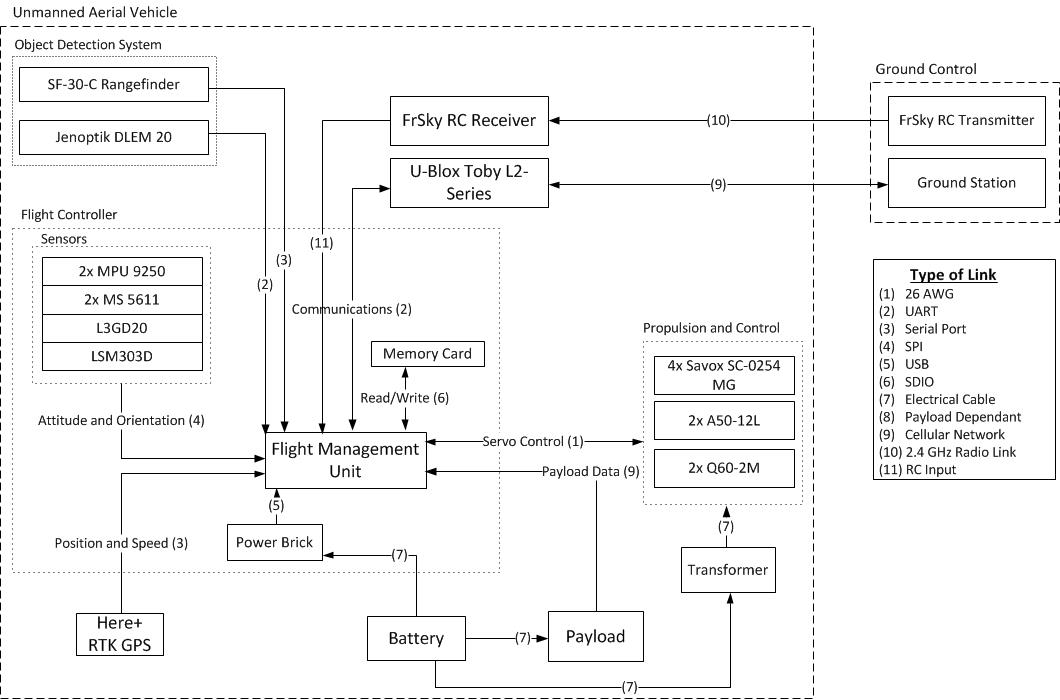
\includegraphics[width=.7\textwidth]{./CommandDataHandling/Figures/HWdiagram.jpg}
    \caption{Hardware Block Diagram}
    \label{fig:hwdia}
\end{figure}

\begin{figure}[ht]
    \centering
    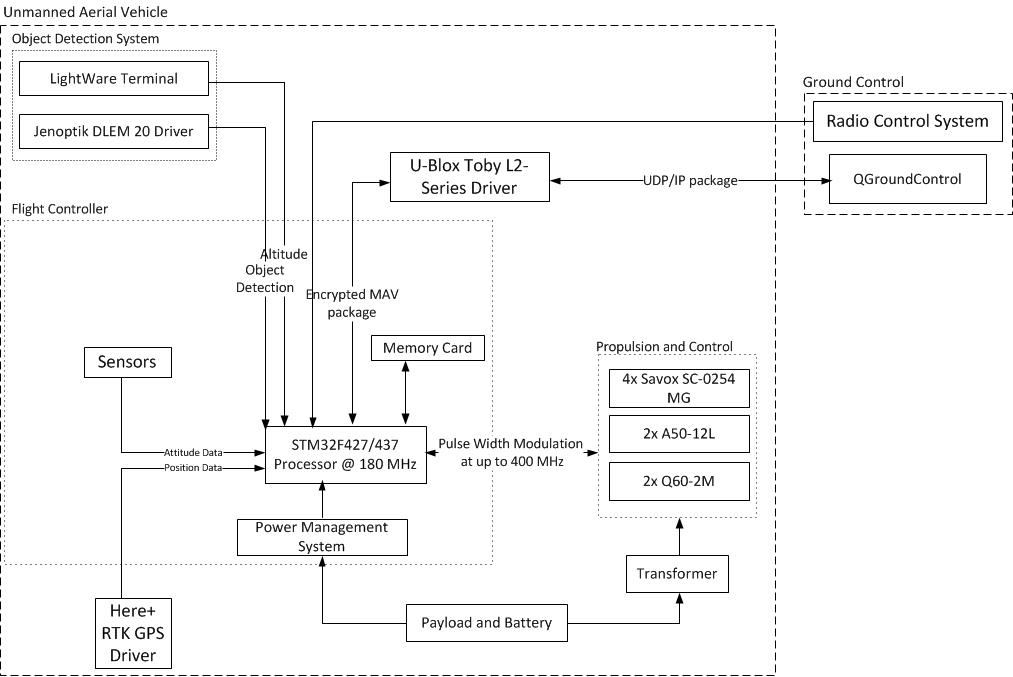
\includegraphics[width=.7\textwidth]{./CommandDataHandling/Figures/SWdiagram.jpg}
    \caption{Software Block Diagram}
    \label{fig:swdia}
\end{figure}

As seen in both diagrams, the central part of the system is the flight management unit. It is the processor used for autonomous flight control and to handle the data inside the system. With the exception of the propulsion and control system, all internal interfaces are connected to it and powered by it. Power related aspects are managed by the power brick. It regulates the voltage and current in order to prevent damage like burnout. It also monitors the power consumption and sends battery specific data to the flight management unit. 
The propulsion and control system in turn is powered by the battery itself. Each engine however has a separate transformer in order to reduce the battery voltage to its operational voltage. The figures show that the engines, actuators and servos used for propulsion and control use a 26 AWG link with PWM technique. The pixhawk 2.1 flight controller has 14 different PWM outputs, eight of them directly controllable by the R/C without need of the flight measurement unit. These will be the four engines used for thrust and the 4 servos used for control. The four tilting actuators are connected via the flight measurement unit. Finally, two more outputs are available in case the droppable payload module is connected for example. 

\section{Electrical Block Diagram}
\label{sec:elec_bloc_diag}



\autoref{fig:elec_diag} shows the electrical block diagram of the UAV system. It includes the different batteries used for power provision, buck converters to regulate the voltage and the different power receivers. Also the cable connectors required for disassembly and assembly are illustrated. As can be seen, the flight controller is just represented as one, more precise information regarding the internal structure can be found in the hardware diagram (\autoref{fig:hwdia}) or the pixhawk 2.1 datasheet \footnote{\url{http://www.unmannedtech.co.uk/uploads/6/7/0/2/6702064/pixhawk_2_25th_july_2016__2_.pdf}, Accessed 21-06-2017}. It was also decided to add two lights to the wing tips in order to make the drone visible in bad conditions. These will adhere to the conventional aircraft colours and hence use a red light on the left side and a green on the right side in order to make it possible to directly recognise the drones flying direction.

Considering the cabling of the system, there are several things that have to be considered during mounting. Firstly, the GPS module is located above the payload in order to receive best satellite signal. Also RC receiver and LTE module will be located here. Then, the flight controller and the other avionics are located in the nose of the fuselage, cabling to this part of the avionics will be minimal in order to avoid electromagnetic interference with the attitude sensors. Then, connections to the wing tips are needed for ailleron control, lights and speed sensor. The fuselage has an empty section above the payload department, which makes it possible to route cables through here. Then, through the wing, the cables can be routed through the shallow carbon tube. 
\begin{figure}[htb]
    \centering
    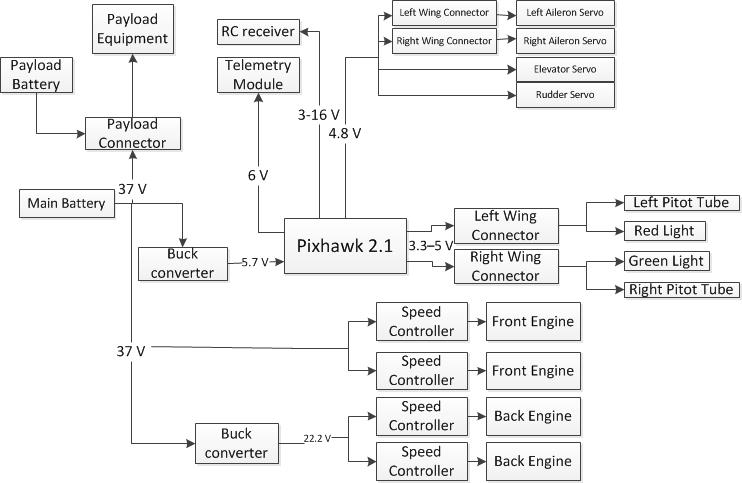
\includegraphics[width=.7\textwidth]{./CommandDataHandling/Figures/elecdiag.jpg}
    \caption{Electrical Block Diagram}
    \label{fig:elec_diag}
\end{figure}


